% Options for packages loaded elsewhere
\PassOptionsToPackage{unicode}{hyperref}
\PassOptionsToPackage{hyphens}{url}
\PassOptionsToPackage{dvipsnames,svgnames,x11names}{xcolor}
%
\documentclass[
  letterpaper,
  DIV=11,
  numbers=noendperiod]{scrartcl}

\usepackage{amsmath,amssymb}
\usepackage{iftex}
\ifPDFTeX
  \usepackage[T1]{fontenc}
  \usepackage[utf8]{inputenc}
  \usepackage{textcomp} % provide euro and other symbols
\else % if luatex or xetex
  \usepackage{unicode-math}
  \defaultfontfeatures{Scale=MatchLowercase}
  \defaultfontfeatures[\rmfamily]{Ligatures=TeX,Scale=1}
\fi
\usepackage{lmodern}
\ifPDFTeX\else  
    % xetex/luatex font selection
\fi
% Use upquote if available, for straight quotes in verbatim environments
\IfFileExists{upquote.sty}{\usepackage{upquote}}{}
\IfFileExists{microtype.sty}{% use microtype if available
  \usepackage[]{microtype}
  \UseMicrotypeSet[protrusion]{basicmath} % disable protrusion for tt fonts
}{}
\makeatletter
\@ifundefined{KOMAClassName}{% if non-KOMA class
  \IfFileExists{parskip.sty}{%
    \usepackage{parskip}
  }{% else
    \setlength{\parindent}{0pt}
    \setlength{\parskip}{6pt plus 2pt minus 1pt}}
}{% if KOMA class
  \KOMAoptions{parskip=half}}
\makeatother
\usepackage{xcolor}
\setlength{\emergencystretch}{3em} % prevent overfull lines
\setcounter{secnumdepth}{5}
% Make \paragraph and \subparagraph free-standing
\ifx\paragraph\undefined\else
  \let\oldparagraph\paragraph
  \renewcommand{\paragraph}[1]{\oldparagraph{#1}\mbox{}}
\fi
\ifx\subparagraph\undefined\else
  \let\oldsubparagraph\subparagraph
  \renewcommand{\subparagraph}[1]{\oldsubparagraph{#1}\mbox{}}
\fi

\usepackage{color}
\usepackage{fancyvrb}
\newcommand{\VerbBar}{|}
\newcommand{\VERB}{\Verb[commandchars=\\\{\}]}
\DefineVerbatimEnvironment{Highlighting}{Verbatim}{commandchars=\\\{\}}
% Add ',fontsize=\small' for more characters per line
\usepackage{framed}
\definecolor{shadecolor}{RGB}{241,243,245}
\newenvironment{Shaded}{\begin{snugshade}}{\end{snugshade}}
\newcommand{\AlertTok}[1]{\textcolor[rgb]{0.68,0.00,0.00}{#1}}
\newcommand{\AnnotationTok}[1]{\textcolor[rgb]{0.37,0.37,0.37}{#1}}
\newcommand{\AttributeTok}[1]{\textcolor[rgb]{0.40,0.45,0.13}{#1}}
\newcommand{\BaseNTok}[1]{\textcolor[rgb]{0.68,0.00,0.00}{#1}}
\newcommand{\BuiltInTok}[1]{\textcolor[rgb]{0.00,0.23,0.31}{#1}}
\newcommand{\CharTok}[1]{\textcolor[rgb]{0.13,0.47,0.30}{#1}}
\newcommand{\CommentTok}[1]{\textcolor[rgb]{0.37,0.37,0.37}{#1}}
\newcommand{\CommentVarTok}[1]{\textcolor[rgb]{0.37,0.37,0.37}{\textit{#1}}}
\newcommand{\ConstantTok}[1]{\textcolor[rgb]{0.56,0.35,0.01}{#1}}
\newcommand{\ControlFlowTok}[1]{\textcolor[rgb]{0.00,0.23,0.31}{#1}}
\newcommand{\DataTypeTok}[1]{\textcolor[rgb]{0.68,0.00,0.00}{#1}}
\newcommand{\DecValTok}[1]{\textcolor[rgb]{0.68,0.00,0.00}{#1}}
\newcommand{\DocumentationTok}[1]{\textcolor[rgb]{0.37,0.37,0.37}{\textit{#1}}}
\newcommand{\ErrorTok}[1]{\textcolor[rgb]{0.68,0.00,0.00}{#1}}
\newcommand{\ExtensionTok}[1]{\textcolor[rgb]{0.00,0.23,0.31}{#1}}
\newcommand{\FloatTok}[1]{\textcolor[rgb]{0.68,0.00,0.00}{#1}}
\newcommand{\FunctionTok}[1]{\textcolor[rgb]{0.28,0.35,0.67}{#1}}
\newcommand{\ImportTok}[1]{\textcolor[rgb]{0.00,0.46,0.62}{#1}}
\newcommand{\InformationTok}[1]{\textcolor[rgb]{0.37,0.37,0.37}{#1}}
\newcommand{\KeywordTok}[1]{\textcolor[rgb]{0.00,0.23,0.31}{#1}}
\newcommand{\NormalTok}[1]{\textcolor[rgb]{0.00,0.23,0.31}{#1}}
\newcommand{\OperatorTok}[1]{\textcolor[rgb]{0.37,0.37,0.37}{#1}}
\newcommand{\OtherTok}[1]{\textcolor[rgb]{0.00,0.23,0.31}{#1}}
\newcommand{\PreprocessorTok}[1]{\textcolor[rgb]{0.68,0.00,0.00}{#1}}
\newcommand{\RegionMarkerTok}[1]{\textcolor[rgb]{0.00,0.23,0.31}{#1}}
\newcommand{\SpecialCharTok}[1]{\textcolor[rgb]{0.37,0.37,0.37}{#1}}
\newcommand{\SpecialStringTok}[1]{\textcolor[rgb]{0.13,0.47,0.30}{#1}}
\newcommand{\StringTok}[1]{\textcolor[rgb]{0.13,0.47,0.30}{#1}}
\newcommand{\VariableTok}[1]{\textcolor[rgb]{0.07,0.07,0.07}{#1}}
\newcommand{\VerbatimStringTok}[1]{\textcolor[rgb]{0.13,0.47,0.30}{#1}}
\newcommand{\WarningTok}[1]{\textcolor[rgb]{0.37,0.37,0.37}{\textit{#1}}}

\providecommand{\tightlist}{%
  \setlength{\itemsep}{0pt}\setlength{\parskip}{0pt}}\usepackage{longtable,booktabs,array}
\usepackage{calc} % for calculating minipage widths
% Correct order of tables after \paragraph or \subparagraph
\usepackage{etoolbox}
\makeatletter
\patchcmd\longtable{\par}{\if@noskipsec\mbox{}\fi\par}{}{}
\makeatother
% Allow footnotes in longtable head/foot
\IfFileExists{footnotehyper.sty}{\usepackage{footnotehyper}}{\usepackage{footnote}}
\makesavenoteenv{longtable}
\usepackage{graphicx}
\makeatletter
\def\maxwidth{\ifdim\Gin@nat@width>\linewidth\linewidth\else\Gin@nat@width\fi}
\def\maxheight{\ifdim\Gin@nat@height>\textheight\textheight\else\Gin@nat@height\fi}
\makeatother
% Scale images if necessary, so that they will not overflow the page
% margins by default, and it is still possible to overwrite the defaults
% using explicit options in \includegraphics[width, height, ...]{}
\setkeys{Gin}{width=\maxwidth,height=\maxheight,keepaspectratio}
% Set default figure placement to htbp
\makeatletter
\def\fps@figure{htbp}
\makeatother

\KOMAoption{captions}{tableheading}
\makeatletter
\@ifpackageloaded{caption}{}{\usepackage{caption}}
\AtBeginDocument{%
\ifdefined\contentsname
  \renewcommand*\contentsname{Table of contents}
\else
  \newcommand\contentsname{Table of contents}
\fi
\ifdefined\listfigurename
  \renewcommand*\listfigurename{List of Figures}
\else
  \newcommand\listfigurename{List of Figures}
\fi
\ifdefined\listtablename
  \renewcommand*\listtablename{List of Tables}
\else
  \newcommand\listtablename{List of Tables}
\fi
\ifdefined\figurename
  \renewcommand*\figurename{Figure}
\else
  \newcommand\figurename{Figure}
\fi
\ifdefined\tablename
  \renewcommand*\tablename{Table}
\else
  \newcommand\tablename{Table}
\fi
}
\@ifpackageloaded{float}{}{\usepackage{float}}
\floatstyle{ruled}
\@ifundefined{c@chapter}{\newfloat{codelisting}{h}{lop}}{\newfloat{codelisting}{h}{lop}[chapter]}
\floatname{codelisting}{Listing}
\newcommand*\listoflistings{\listof{codelisting}{List of Listings}}
\makeatother
\makeatletter
\makeatother
\makeatletter
\@ifpackageloaded{caption}{}{\usepackage{caption}}
\@ifpackageloaded{subcaption}{}{\usepackage{subcaption}}
\makeatother
\ifLuaTeX
  \usepackage{selnolig}  % disable illegal ligatures
\fi
\usepackage{bookmark}

\IfFileExists{xurl.sty}{\usepackage{xurl}}{} % add URL line breaks if available
\urlstyle{same} % disable monospaced font for URLs
\hypersetup{
  pdftitle={STAT-427/627 Final 24S},
  colorlinks=true,
  linkcolor={blue},
  filecolor={Maroon},
  citecolor={Blue},
  urlcolor={Blue},
  pdfcreator={LaTeX via pandoc}}

\title{STAT-427/627 Final 24S}
\usepackage{etoolbox}
\makeatletter
\providecommand{\subtitle}[1]{% add subtitle to \maketitle
  \apptocmd{\@title}{\par {\large #1 \par}}{}{}
}
\makeatother
\subtitle{Name\_\_\_\_\_\_\_\_\_\_\_\_\_\_\_\_\_\_\_\_\_\_\_\_\_\_\_\_\_\_\_Course\_\_\_\_\_\_\_\_\_\_\_\_\_}
\author{}
\date{}

\begin{document}
\maketitle

Be brief but show your reasoning (partial credit?). \textbf{Label your
work and answers for each problem if on a different page.} Put your name
on each piece of paper. You can use your notes, textbook, calculator,
and computer and the internet to access course materials.

\begin{itemize}
\item
  Recommend you do the problem one plots on paper instead of taking the
  time to code. Turn in the paper and as an option, you con take a
  picture and put the file in the same folder as your code file. Use the
  following rmarkdown syntax at the appropriate location to embed the
  file into your output. \includegraphics{myfile.png}.
\item
  Each problem is 20 points. Total points = 40. Time = 2 hr 30 min.
\end{itemize}

\section{Insurance Predictions: Do by
hand.}\label{insurance-predictions-do-by-hand.}

An insurance company wants to predict if a new customer will have a
major operation within 10 years. They select 11 customers at random as
training data to predict an operation based on the customer's age and
their average annual cost of medical care.

\begin{longtable}[]{@{}
  >{\raggedright\arraybackslash}p{(\columnwidth - 22\tabcolsep) * \real{0.2466}}
  >{\centering\arraybackslash}p{(\columnwidth - 22\tabcolsep) * \real{0.0685}}
  >{\centering\arraybackslash}p{(\columnwidth - 22\tabcolsep) * \real{0.0685}}
  >{\centering\arraybackslash}p{(\columnwidth - 22\tabcolsep) * \real{0.0685}}
  >{\centering\arraybackslash}p{(\columnwidth - 22\tabcolsep) * \real{0.0685}}
  >{\centering\arraybackslash}p{(\columnwidth - 22\tabcolsep) * \real{0.0685}}
  >{\centering\arraybackslash}p{(\columnwidth - 22\tabcolsep) * \real{0.0685}}
  >{\centering\arraybackslash}p{(\columnwidth - 22\tabcolsep) * \real{0.0685}}
  >{\centering\arraybackslash}p{(\columnwidth - 22\tabcolsep) * \real{0.0685}}
  >{\centering\arraybackslash}p{(\columnwidth - 22\tabcolsep) * \real{0.0685}}
  >{\centering\arraybackslash}p{(\columnwidth - 22\tabcolsep) * \real{0.0685}}
  >{\centering\arraybackslash}p{(\columnwidth - 22\tabcolsep) * \real{0.0685}}@{}}
\toprule\noalign{}
\begin{minipage}[b]{\linewidth}\raggedright
Person
\end{minipage} & \begin{minipage}[b]{\linewidth}\centering
A
\end{minipage} & \begin{minipage}[b]{\linewidth}\centering
B
\end{minipage} & \begin{minipage}[b]{\linewidth}\centering
C
\end{minipage} & \begin{minipage}[b]{\linewidth}\centering
D
\end{minipage} & \begin{minipage}[b]{\linewidth}\centering
E
\end{minipage} & \begin{minipage}[b]{\linewidth}\centering
F
\end{minipage} & \begin{minipage}[b]{\linewidth}\centering
G
\end{minipage} & \begin{minipage}[b]{\linewidth}\centering
H
\end{minipage} & \begin{minipage}[b]{\linewidth}\centering
I
\end{minipage} & \begin{minipage}[b]{\linewidth}\centering
J
\end{minipage} & \begin{minipage}[b]{\linewidth}\centering
K
\end{minipage} \\
\midrule\noalign{}
\endhead
\bottomrule\noalign{}
\endlastfoot
Age & 20 & 22 & 23 & 24 & 25 & 26 & 27 & 29 & 32 & 35 & 37 \\
Average Cost & 5 & 11 & 8 & 9 & 15 & 19 & 24 & 21 & 18 & 20 & 17 \\
Had an Operation & N & Y & N & N & N & Y & Y & N & N & Y & Y \\
\end{longtable}

To classify future insured, the company partitions its predictor space
(Age, Cost) as on the right (see hard copy).

(a) Plot the persons \emph{using their label} on the partition plot.

\begin{itemize}
\tightlist
\item
  Draw a classification tree that corresponds to this partition.
\item
  At each internal node, state the splitting condition and threshold.
\item
  At each terminal (leaf) node, state the predicted response.
\end{itemize}

(b) Fill in the following table with the prediction for each point based
on your tree.

\begin{itemize}
\tightlist
\item
  Fill out the confusion matrix.
\item
  Calculate the \emph{training} classification rate from the confusion
  matrix.
\end{itemize}

\begin{longtable}[]{@{}
  >{\raggedright\arraybackslash}p{(\columnwidth - 22\tabcolsep) * \real{0.2466}}
  >{\centering\arraybackslash}p{(\columnwidth - 22\tabcolsep) * \real{0.0685}}
  >{\centering\arraybackslash}p{(\columnwidth - 22\tabcolsep) * \real{0.0685}}
  >{\centering\arraybackslash}p{(\columnwidth - 22\tabcolsep) * \real{0.0685}}
  >{\centering\arraybackslash}p{(\columnwidth - 22\tabcolsep) * \real{0.0685}}
  >{\centering\arraybackslash}p{(\columnwidth - 22\tabcolsep) * \real{0.0685}}
  >{\centering\arraybackslash}p{(\columnwidth - 22\tabcolsep) * \real{0.0685}}
  >{\centering\arraybackslash}p{(\columnwidth - 22\tabcolsep) * \real{0.0685}}
  >{\centering\arraybackslash}p{(\columnwidth - 22\tabcolsep) * \real{0.0685}}
  >{\centering\arraybackslash}p{(\columnwidth - 22\tabcolsep) * \real{0.0685}}
  >{\centering\arraybackslash}p{(\columnwidth - 22\tabcolsep) * \real{0.0685}}
  >{\centering\arraybackslash}p{(\columnwidth - 22\tabcolsep) * \real{0.0685}}@{}}
\toprule\noalign{}
\begin{minipage}[b]{\linewidth}\raggedright
Person
\end{minipage} & \begin{minipage}[b]{\linewidth}\centering
A
\end{minipage} & \begin{minipage}[b]{\linewidth}\centering
B
\end{minipage} & \begin{minipage}[b]{\linewidth}\centering
C
\end{minipage} & \begin{minipage}[b]{\linewidth}\centering
D
\end{minipage} & \begin{minipage}[b]{\linewidth}\centering
E
\end{minipage} & \begin{minipage}[b]{\linewidth}\centering
F
\end{minipage} & \begin{minipage}[b]{\linewidth}\centering
G
\end{minipage} & \begin{minipage}[b]{\linewidth}\centering
H
\end{minipage} & \begin{minipage}[b]{\linewidth}\centering
I
\end{minipage} & \begin{minipage}[b]{\linewidth}\centering
J
\end{minipage} & \begin{minipage}[b]{\linewidth}\centering
K
\end{minipage} \\
\midrule\noalign{}
\endhead
\bottomrule\noalign{}
\endlastfoot
Age & 20 & 22 & 23 & 24 & 25 & 26 & 27 & 29 & 32 & 35 & 37 \\
Average Cost & 5 & 11 & 8 & 9 & 15 & 19 & 24 & 21 & 18 & 20 & 17 \\
Had an Operation & N & Y & N & N & N & Y & Y & N & N & Y & Y \\
Prediction? & & & & & & & & & & & \\
\end{longtable}

\begin{longtable}[]{@{}ccc@{}}
\toprule\noalign{}
\endhead
\bottomrule\noalign{}
\endlastfoot
& Pred Yes & Pred No \\
Actual-Yes & & \\
Actual-No & & \\
\end{longtable}

\begin{itemize}
\tightlist
\item
  Classification Rate?
\end{itemize}

(c) A random forest is constructed for the same data. It has 3 trees and
each is pruned to 1 split with 2 terminal nodes:

\begin{itemize}
\tightlist
\item
  The 1st tree sample is persons A, C, C, D, E, E, F, F, F, G, I. It
  splits on Cost.
\item
  The 2nd tree sample is persons A, C, D, D, E, F, F, G, G, H, K. It
  splits on Age.
\item
  The 3rd tree sample is persons A, A, D, D, E, E, F, G, J, K, K. It
  splits on Cost.
\end{itemize}

The following table summarizes the data for the forest.

\begin{longtable}[]{@{}
  >{\raggedright\arraybackslash}p{(\columnwidth - 22\tabcolsep) * \real{0.2466}}
  >{\centering\arraybackslash}p{(\columnwidth - 22\tabcolsep) * \real{0.0685}}
  >{\centering\arraybackslash}p{(\columnwidth - 22\tabcolsep) * \real{0.0685}}
  >{\centering\arraybackslash}p{(\columnwidth - 22\tabcolsep) * \real{0.0685}}
  >{\centering\arraybackslash}p{(\columnwidth - 22\tabcolsep) * \real{0.0685}}
  >{\centering\arraybackslash}p{(\columnwidth - 22\tabcolsep) * \real{0.0685}}
  >{\centering\arraybackslash}p{(\columnwidth - 22\tabcolsep) * \real{0.0685}}
  >{\centering\arraybackslash}p{(\columnwidth - 22\tabcolsep) * \real{0.0685}}
  >{\centering\arraybackslash}p{(\columnwidth - 22\tabcolsep) * \real{0.0685}}
  >{\centering\arraybackslash}p{(\columnwidth - 22\tabcolsep) * \real{0.0685}}
  >{\centering\arraybackslash}p{(\columnwidth - 22\tabcolsep) * \real{0.0685}}
  >{\centering\arraybackslash}p{(\columnwidth - 22\tabcolsep) * \real{0.0685}}@{}}
\toprule\noalign{}
\begin{minipage}[b]{\linewidth}\raggedright
Person
\end{minipage} & \begin{minipage}[b]{\linewidth}\centering
A
\end{minipage} & \begin{minipage}[b]{\linewidth}\centering
B
\end{minipage} & \begin{minipage}[b]{\linewidth}\centering
C
\end{minipage} & \begin{minipage}[b]{\linewidth}\centering
D
\end{minipage} & \begin{minipage}[b]{\linewidth}\centering
E
\end{minipage} & \begin{minipage}[b]{\linewidth}\centering
F
\end{minipage} & \begin{minipage}[b]{\linewidth}\centering
G
\end{minipage} & \begin{minipage}[b]{\linewidth}\centering
H
\end{minipage} & \begin{minipage}[b]{\linewidth}\centering
I
\end{minipage} & \begin{minipage}[b]{\linewidth}\centering
J
\end{minipage} & \begin{minipage}[b]{\linewidth}\centering
K
\end{minipage} \\
\midrule\noalign{}
\endhead
\bottomrule\noalign{}
\endlastfoot
Age & 20 & 22 & 23 & 24 & 25 & 26 & 27 & 29 & 32 & 35 & 37 \\
Average Cost & 5 & 11 & 8 & 9 & 15 & 19 & 24 & 21 & 18 & 20 & 17 \\
Had an Operation & N & Y & N & N & N & Y & Y & N & N & Y & Y \\
Tree 1 & 1 & & 2 & 1 & 2 & 3 & 1 & & 1 & & \\
Tree 2 & 1 & & 1 & 2 & 1 & 2 & 2 & 1 & & & 1 \\
Tree 3 & 2 & & & 2 & 2 & 1 & 1 & & & 1 & 2 \\
\end{longtable}

\begin{itemize}
\tightlist
\item
  In the following plots, put a number next to each point for how many
  times it is in the tree and line through the Out-Of-Bag points
\item
  For each tree, draw a single partition for the given variable at the
  threshold which creates the terminal nodes as pure as possible.
\item
  Below the three plots, for each tree, indicate the number of pure
  nodes (if any) for each tree and your calculation of the threshold
  value based on the closest points on either side of the threshold. You
  do \textbf{not} need to calculate the Gini impurity index.
\item
  For each tree, plot a New customer with age 26 with an average cost of
  18.
\item
  Use this random forest to predict whether the New customer will have
  an operation and explain your reasoning for the prediction.
\end{itemize}

Number of pure nodes, Threshold, and Prediction for each tree?

The 1\textsuperscript{st} tree:

The 2\textsuperscript{nd} tree:

The 3\textsuperscript{rd} tree:

Overall Prediction for the new Customer and Rationale:

(d) (STAT-627 only) Calculate the \emph{prediction} error rate of the
random forest in question (c), using out-of-bag (OOB) data.

\begin{itemize}
\tightlist
\item
  Using your thresholds from part (c), fill in the following table with
  the predictions for only the OOB persons in each tree.
\item
  Calculate the overall OOB prediction for each OOB person.
\item
  Indicate if each overall OOB prediction is an error or not (1, 0).
\item
  Calculate the prediction error rate.
\item
  What would you recommend to improve the prediction error rate?
\end{itemize}

\begin{longtable}[]{@{}
  >{\raggedright\arraybackslash}p{(\columnwidth - 22\tabcolsep) * \real{0.2466}}
  >{\centering\arraybackslash}p{(\columnwidth - 22\tabcolsep) * \real{0.0685}}
  >{\centering\arraybackslash}p{(\columnwidth - 22\tabcolsep) * \real{0.0685}}
  >{\centering\arraybackslash}p{(\columnwidth - 22\tabcolsep) * \real{0.0685}}
  >{\centering\arraybackslash}p{(\columnwidth - 22\tabcolsep) * \real{0.0685}}
  >{\centering\arraybackslash}p{(\columnwidth - 22\tabcolsep) * \real{0.0685}}
  >{\centering\arraybackslash}p{(\columnwidth - 22\tabcolsep) * \real{0.0685}}
  >{\centering\arraybackslash}p{(\columnwidth - 22\tabcolsep) * \real{0.0685}}
  >{\centering\arraybackslash}p{(\columnwidth - 22\tabcolsep) * \real{0.0685}}
  >{\centering\arraybackslash}p{(\columnwidth - 22\tabcolsep) * \real{0.0685}}
  >{\centering\arraybackslash}p{(\columnwidth - 22\tabcolsep) * \real{0.0685}}
  >{\centering\arraybackslash}p{(\columnwidth - 22\tabcolsep) * \real{0.0685}}@{}}
\toprule\noalign{}
\begin{minipage}[b]{\linewidth}\raggedright
Person
\end{minipage} & \begin{minipage}[b]{\linewidth}\centering
A
\end{minipage} & \begin{minipage}[b]{\linewidth}\centering
B
\end{minipage} & \begin{minipage}[b]{\linewidth}\centering
C
\end{minipage} & \begin{minipage}[b]{\linewidth}\centering
D
\end{minipage} & \begin{minipage}[b]{\linewidth}\centering
E
\end{minipage} & \begin{minipage}[b]{\linewidth}\centering
F
\end{minipage} & \begin{minipage}[b]{\linewidth}\centering
G
\end{minipage} & \begin{minipage}[b]{\linewidth}\centering
H
\end{minipage} & \begin{minipage}[b]{\linewidth}\centering
I
\end{minipage} & \begin{minipage}[b]{\linewidth}\centering
J
\end{minipage} & \begin{minipage}[b]{\linewidth}\centering
K
\end{minipage} \\
\midrule\noalign{}
\endhead
\bottomrule\noalign{}
\endlastfoot
Tree 1 & & & & & & & & & & & \\
Tree 2 & & & & & & & & & & & \\
Tree 3 & & & & & & & & & & & \\
------------------ & --- & --- & --- & --- & --- & --- & --- & -- & ---
& --- & --- \\
Predicted & & & & & & & & & & & \\
Had an Operation & N & Y & N & N & N & Y & Y & N & N & Y & Y \\
Error? & & & & & & & & & & & \\
\end{longtable}

(e) Is there a \emph{maximal margin} classifier for this dataset?
Explain your answer. Consider drawing some lines on the scatterplot you
created in (a).

(f) Consider the following plot from an SVM classifier. (see hard copy)

\begin{itemize}
\tightlist
\item
  How many support vectors are there?
\item
  What type of kernel is being used based on the plot and why?
\item
  What is the training classification rate?
\end{itemize}

\section{College Scorecard Data}\label{college-scorecard-data}

The US Department of Education collects data from every ``college''
level institution in America and makes a lot of data available under the
\href{https://collegescorecard.ed.gov/}{College Scorecard}.

\begin{itemize}
\tightlist
\item
  This question uses a curated extract of the college scorecard data.
  The variable names and definitions are at the end.
\item
  This dataset has 23 variables of data on 1,695 four-year colleges.
\item
  This dataset is on Canvas or at
  ``https://raw.githubusercontent.com/AU-datascience/data/main/427-627/college\_scorecard\_extract\_sep\_2023.csv''.
\end{itemize}

We want to predict the Endowment of a new colleges given the other
variables as potential predictors.

In the following steps, build models to predict the College Endowment
(\texttt{ENDOWBEGIN}) and use \(K=10\)-fold cross-validation to tune and
evaluate predictive performance with \textbf{\texttt{set.seed(123)} as
appropriate.}

\begin{itemize}
\item
  For each problem, describe your approach, your R code, the most
  important results, and your interpretation of the results.
\item
  You may write your responses on this document by hand after running
  code in R and/or submit a file on Canvas with your approach, code,
  results, and interpretation of results.
\end{itemize}

\subsection{Multiple Linear Regression
Regularization}\label{multiple-linear-regression-regularization}

\begin{itemize}
\tightlist
\item
  Load the data and assign the name \texttt{college} to it. Get rid of
  any records with \texttt{NA}s and divided \texttt{ENDOWBEGIN} by 1
  million to reduce the scale. Glimpse \texttt{college}.
\end{itemize}

\begin{Shaded}
\begin{Highlighting}[]
\FunctionTok{library}\NormalTok{(tidyverse)}
\NormalTok{college }\OtherTok{\textless{}{-}} \FunctionTok{read\_csv}\NormalTok{(}\StringTok{"https://raw.githubusercontent.com/AU{-}datascience/data/main/427{-}627/college\_scorecard\_extract\_sep\_2023.csv"}\NormalTok{)}
\NormalTok{college }\OtherTok{\textless{}{-}} \FunctionTok{na.omit}\NormalTok{(college)}
\NormalTok{college}\SpecialCharTok{$}\NormalTok{ENDOWBEGIN }\OtherTok{\textless{}{-}}\NormalTok{ college}\SpecialCharTok{$}\NormalTok{ENDOWBEGIN}\SpecialCharTok{/}\DecValTok{1000000}
\CommentTok{\#college \textless{}{-} read\_csv("./data/college\_scorecard\_extract\_sep\_2023.csv")}
\CommentTok{\#glimpse(college) }
\end{Highlighting}
\end{Shaded}

\begin{itemize}
\tightlist
\item
  Fit a multiple linear regression of Endowment (\(ENDOWBEGIN\)) on all
  the other variables as a full model.
\end{itemize}

\begin{Shaded}
\begin{Highlighting}[]
\NormalTok{full\_model }\OtherTok{\textless{}{-}} \FunctionTok{lm}\NormalTok{(ENDOWBEGIN }\SpecialCharTok{\textasciitilde{}}\NormalTok{ ., }\AttributeTok{data =}\NormalTok{ college)}
\end{Highlighting}
\end{Shaded}

\begin{itemize}
\tightlist
\item
  How many predictors appear important with a \(p\) value less than 0.1?
\end{itemize}

\begin{Shaded}
\begin{Highlighting}[]
\FunctionTok{summary}\NormalTok{(full\_model)}
\end{Highlighting}
\end{Shaded}

\begin{verbatim}

Call:
lm(formula = ENDOWBEGIN ~ ., data = college)

Residuals:
    Min      1Q  Median      3Q     Max 
-8188.4  -539.3    34.9   550.2 24097.4 

Coefficients:
                         Estimate Std. Error t value Pr(>|t|)    
(Intercept)             2.026e+03  3.178e+03   0.638  0.52391    
ADM_RATE               -1.061e+03  3.767e+02  -2.817  0.00495 ** 
AGE_ENTRY              -7.333e+01  3.757e+01  -1.952  0.05126 .  
AVGFACSAL               4.364e-01  5.233e-02   8.340 2.82e-16 ***
CONTROLPublic          -1.116e+03  2.583e+02  -4.321 1.73e-05 ***
COSTT4_A               -1.598e-02  8.728e-03  -1.831  0.06748 .  
FEMALE                 -2.365e+02  7.230e+02  -0.327  0.74369    
FIRST_GEN               3.077e+03  1.237e+03   2.488  0.01304 *  
GRAD_DEBT_MDN          -4.500e-02  2.169e-02  -2.075  0.03828 *  
LOCALERural             3.976e+02  3.162e+02   1.257  0.20891    
LOCALESurbuban         -6.201e+01  1.474e+02  -0.421  0.67402    
LOCALETown              1.868e+02  1.613e+02   1.158  0.24714    
MD_EARN_WNE_P10        -1.483e-01  1.314e-02 -11.286  < 2e-16 ***
MN_EARN_WNE_P10         1.849e-01  1.294e-02  14.284  < 2e-16 ***
PCIP14                 -1.033e+03  8.105e+02  -1.274  0.20294    
PCIP27                  2.016e+04  4.720e+03   4.272 2.15e-05 ***
PFTFAC                  3.843e+01  2.756e+02   0.139  0.88912    
PCT_ASIAN              -7.123e+01  5.362e+01  -1.329  0.18435    
PCT_BLACK              -2.858e+00  2.909e+01  -0.098  0.92177    
PCT_WHITE              -1.642e+00  2.798e+01  -0.059  0.95321    
PCT_HISPANIC           -2.789e+01  1.228e+01  -2.271  0.02338 *  
PCTPELL                 5.174e+02  7.835e+02   0.660  0.50917    
REGIONGreat Lakes      -4.843e+02  3.646e+02  -1.328  0.18441    
REGIONMid-East         -8.869e+02  3.457e+02  -2.566  0.01046 *  
REGIONNew England      -8.037e+02  3.856e+02  -2.084  0.03742 *  
REGIONOutlying Regions -9.732e+02  1.748e+03  -0.557  0.57791    
REGIONPLains           -4.136e+02  3.708e+02  -1.115  0.26501    
REGIONRocky Mountains  -5.710e+02  4.615e+02  -1.237  0.21634    
REGIONSoutheast        -6.046e+02  3.867e+02  -1.563  0.11832    
REGIONSouthwest        -5.571e+02  3.730e+02  -1.493  0.13568    
SAT_AVG                -2.030e+00  1.172e+00  -1.732  0.08362 .  
UGDS                    1.666e-02  1.002e-02   1.663  0.09672 .  
---
Signif. codes:  0 '***' 0.001 '**' 0.01 '*' 0.05 '.' 0.1 ' ' 1

Residual standard error: 1690 on 887 degrees of freedom
Multiple R-squared:  0.5486,    Adjusted R-squared:  0.5328 
F-statistic: 34.77 on 31 and 887 DF,  p-value: < 2.2e-16
\end{verbatim}

there are 6 predictors with atleast 2 stars so their p-values are less
than 0.01.

\begin{itemize}
\tightlist
\item
  Which of those increase the endowment? AVGFACSAL, MN\_EARN\_WNE\_P10,
  and PCIP27
\end{itemize}

Do any of the variables have a high generalized variance inflation
factor GVIF? If any, which ones and do they make sense as having high
GVIF given the other variables?

\begin{Shaded}
\begin{Highlighting}[]
\FunctionTok{library}\NormalTok{(car)}
\end{Highlighting}
\end{Shaded}

\begin{verbatim}
Loading required package: carData
\end{verbatim}

\begin{verbatim}

Attaching package: 'car'
\end{verbatim}

\begin{verbatim}
The following object is masked from 'package:dplyr':

    recode
\end{verbatim}

\begin{verbatim}
The following object is masked from 'package:purrr':

    some
\end{verbatim}

\begin{Shaded}
\begin{Highlighting}[]
\NormalTok{vif\_values }\OtherTok{\textless{}{-}} \FunctionTok{vif}\NormalTok{(full\_model)}
\NormalTok{vif\_values}
\end{Highlighting}
\end{Shaded}

\begin{verbatim}
                     GVIF Df GVIF^(1/(2*Df))
ADM_RATE         1.956409  1        1.398717
AGE_ENTRY        2.362937  1        1.537185
AVGFACSAL        5.856266  1        2.419972
CONTROL          5.087335  1        2.255512
COSTT4_A         7.482394  1        2.735396
FEMALE           1.812391  1        1.346251
FIRST_GEN        4.281285  1        2.069127
GRAD_DEBT_MDN    1.957953  1        1.399269
LOCALE           1.663459  3        1.088517
MD_EARN_WNE_P10 11.123241  1        3.335152
MN_EARN_WNE_P10 11.799559  1        3.435049
PCIP14           1.990121  1        1.410716
PCIP27           1.642977  1        1.281787
PFTFAC           1.208391  1        1.099268
PCT_ASIAN        7.129318  1        2.670078
PCT_BLACK       32.073927  1        5.663385
PCT_WHITE       36.596033  1        6.049465
PCT_HISPANIC     3.223241  1        1.795339
PCTPELL          3.383407  1        1.839404
REGION          11.251857  8        1.163326
SAT_AVG          7.508675  1        2.740196
UGDS             2.070544  1        1.438939
\end{verbatim}

using 5 as my GVIF threshold, it appears the following variables may be
subject to multicollinearity: AVGFACSAL, CONTROL, COSTT4\_A,
MD\_EARN\_WNE\_P10, MN\_EARN\_WNE\_P10, PCT\_BLACK, PCT\_ASIAN,
PCT\_WHITE, REGION, SAT\_AVG

Refit a reduced model without \texttt{MN\_EARN\_WNE\_P10} and
\texttt{PCT\_WHITE}. Are there any changes in significant variables?

\begin{Shaded}
\begin{Highlighting}[]
\NormalTok{reduced\_model }\OtherTok{\textless{}{-}} \FunctionTok{lm}\NormalTok{(ENDOWBEGIN }\SpecialCharTok{\textasciitilde{}}\NormalTok{ . }\SpecialCharTok{{-}}\NormalTok{ MN\_EARN\_WNE\_P10 }\SpecialCharTok{{-}}\NormalTok{ PCT\_WHITE, }\AttributeTok{data =}\NormalTok{ college)}
\FunctionTok{summary}\NormalTok{(reduced\_model)}
\end{Highlighting}
\end{Shaded}

\begin{verbatim}

Call:
lm(formula = ENDOWBEGIN ~ . - MN_EARN_WNE_P10 - PCT_WHITE, data = college)

Residuals:
    Min      1Q  Median      3Q     Max 
-5325.4  -636.7    -2.7   536.4 29884.2 

Coefficients:
                         Estimate Std. Error t value Pr(>|t|)    
(Intercept)             6.267e+02  2.130e+03   0.294 0.768639    
ADM_RATE               -1.542e+03  4.154e+02  -3.712 0.000219 ***
AGE_ENTRY              -2.647e+01  4.141e+01  -0.639 0.522903    
AVGFACSAL               6.863e-01  5.451e-02  12.592  < 2e-16 ***
CONTROLPublic          -1.388e+03  2.849e+02  -4.871 1.31e-06 ***
COSTT4_A               -1.170e-02  9.621e-03  -1.216 0.224122    
FEMALE                 -1.262e+03  7.966e+02  -1.584 0.113640    
FIRST_GEN               4.448e+03  1.366e+03   3.256 0.001173 ** 
GRAD_DEBT_MDN          -8.266e-02  2.382e-02  -3.470 0.000545 ***
LOCALERural             1.595e+02  3.497e+02   0.456 0.648466    
LOCALESurbuban         -2.191e+02  1.628e+02  -1.346 0.178639    
LOCALETown              1.859e+02  1.778e+02   1.046 0.296020    
MD_EARN_WNE_P10        -2.391e-03  9.089e-03  -0.263 0.792580    
PCIP14                 -2.056e+03  8.931e+02  -2.302 0.021564 *  
PCIP27                  2.310e+04  5.223e+03   4.423 1.09e-05 ***
PFTFAC                 -6.161e+01  3.047e+02  -0.202 0.839820    
PCT_ASIAN              -9.126e+01  3.291e+01  -2.773 0.005672 ** 
PCT_BLACK               9.374e+00  8.745e+00   1.072 0.284044    
PCT_HISPANIC           -3.261e+01  1.075e+01  -3.035 0.002476 ** 
PCTPELL                -1.279e+01  8.670e+02  -0.015 0.988237    
REGIONGreat Lakes      -2.153e+02  3.805e+02  -0.566 0.571559    
REGIONMid-East         -7.678e+02  3.620e+02  -2.121 0.034201 *  
REGIONNew England      -8.115e+02  4.148e+02  -1.956 0.050756 .  
REGIONOutlying Regions -9.512e+02  1.933e+03  -0.492 0.622754    
REGIONPLains           -1.270e+02  3.959e+02  -0.321 0.748422    
REGIONRocky Mountains  -6.060e+01  5.097e+02  -0.119 0.905381    
REGIONSoutheast        -2.466e+02  4.008e+02  -0.615 0.538519    
REGIONSouthwest         4.711e+01  4.106e+02   0.115 0.908679    
SAT_AVG                -1.167e+00  1.296e+00  -0.901 0.368010    
UGDS                    5.020e-04  1.098e-02   0.046 0.963539    
---
Signif. codes:  0 '***' 0.001 '**' 0.01 '*' 0.05 '.' 0.1 ' ' 1

Residual standard error: 1872 on 889 degrees of freedom
Multiple R-squared:  0.4447,    Adjusted R-squared:  0.4266 
F-statistic: 24.55 on 29 and 889 DF,  p-value: < 2.2e-16
\end{verbatim}

now for significant variables we have PCT\_HISPANIC, PCT\_ASIAN, PCIP27,
GRAD\_DEBT\_MDN, FIRST\_GEN, CONTROLPublic, AVGFACSAL, ADM\_RATE

\begin{itemize}
\tightlist
\item
  Check the GVIF again and comment on any changes.
\end{itemize}

\begin{Shaded}
\begin{Highlighting}[]
\FunctionTok{vif}\NormalTok{(reduced\_model)}
\end{Highlighting}
\end{Shaded}

\begin{verbatim}
                    GVIF Df GVIF^(1/(2*Df))
ADM_RATE        1.938564  1        1.392323
AGE_ENTRY       2.339179  1        1.529438
AVGFACSAL       5.177903  1        2.275501
CONTROL         5.040528  1        2.245112
COSTT4_A        7.408387  1        2.721835
FEMALE          1.792726  1        1.338927
FIRST_GEN       4.255414  1        2.062865
GRAD_DEBT_MDN   1.924363  1        1.387214
LOCALE          1.626197  3        1.084415
MD_EARN_WNE_P10 4.338904  1        2.083004
PCIP14          1.968773  1        1.403130
PCIP27          1.639128  1        1.280284
PFTFAC          1.203818  1        1.097186
PCT_ASIAN       2.188334  1        1.479302
PCT_BLACK       2.360766  1        1.536479
PCT_HISPANIC    2.010628  1        1.417966
PCTPELL         3.375700  1        1.837308
REGION          8.191355  8        1.140472
SAT_AVG         7.483227  1        2.735549
UGDS            2.024164  1        1.422731
\end{verbatim}

now for variables subject to multicolinearity we have: AVGFACSAL,
CONTROL, COSTT4\_A, REGION, SAT\_AVG.

\begin{itemize}
\tightlist
\item
  Create a new data frame with the variables below (you can use the
  following code).

  \begin{itemize}
  \tightlist
  \item
    Remove the rows with \texttt{REGION\ =\ "Outlying\ Regions"}.
  \item
    Convert all character variables to factors.
  \end{itemize}
\end{itemize}

\begin{Shaded}
\begin{Highlighting}[]
\NormalTok{college }\SpecialCharTok{|\textgreater{}}
\NormalTok{  dplyr}\SpecialCharTok{::}\FunctionTok{select}\NormalTok{(}
\NormalTok{     ENDOWBEGIN, ADM\_RATE, AVGFACSAL, CONTROL,FIRST\_GEN, GRAD\_DEBT\_MDN, PCIP27, }
\NormalTok{PCT\_ASIAN, REGION}
\NormalTok{  ) }\SpecialCharTok{|\textgreater{}}
  \FunctionTok{filter}\NormalTok{(REGION }\SpecialCharTok{!=} \StringTok{"Outlying Regions"}\NormalTok{) }\SpecialCharTok{|\textgreater{}}
  \FunctionTok{mutate}\NormalTok{(}\FunctionTok{across}\NormalTok{(}\FunctionTok{where}\NormalTok{(is.character), as.factor)) }\OtherTok{{-}\textgreater{}}
\NormalTok{college2}
\end{Highlighting}
\end{Shaded}

\begin{itemize}
\tightlist
\item
  Use the \{boot\} package with \texttt{college2} to report the
  prediction MSE for a full model (\texttt{ENDOWBEGIN} on the other
  data) based on K-10 fold cross-validation adjusted deviance.
\end{itemize}

\begin{Shaded}
\begin{Highlighting}[]
\FunctionTok{library}\NormalTok{(boot)}
\end{Highlighting}
\end{Shaded}

\begin{verbatim}

Attaching package: 'boot'
\end{verbatim}

\begin{verbatim}
The following object is masked from 'package:car':

    logit
\end{verbatim}

\begin{Shaded}
\begin{Highlighting}[]
\FunctionTok{set.seed}\NormalTok{(}\DecValTok{123}\NormalTok{)}

\NormalTok{lm\_full }\OtherTok{\textless{}{-}} \FunctionTok{glm}\NormalTok{(ENDOWBEGIN }\SpecialCharTok{\textasciitilde{}}\NormalTok{ ., }\AttributeTok{data =}\NormalTok{ college2)}

\NormalTok{cv\_error }\OtherTok{\textless{}{-}} \FunctionTok{cv.glm}\NormalTok{(college2, lm\_full, }\AttributeTok{K =} \DecValTok{10}\NormalTok{)}
\NormalTok{cv\_error}\SpecialCharTok{$}\NormalTok{delta[}\DecValTok{1}\NormalTok{]}
\end{Highlighting}
\end{Shaded}

\begin{verbatim}
[1] 3875289
\end{verbatim}

\subsection{Regularization via
Shrinkage}\label{regularization-via-shrinkage}

Use LASSO with cross validation to model \texttt{ENDOWBEGIN} on the
other variables in \texttt{college2} and find the best lambda.

\begin{itemize}
\tightlist
\item
  Create model matrices for \texttt{X} and \texttt{Y}.
\item
  Use \texttt{set.seed(123)} for the cross validation.
\end{itemize}

\begin{Shaded}
\begin{Highlighting}[]
\FunctionTok{library}\NormalTok{(glmnet)}
\end{Highlighting}
\end{Shaded}

\begin{verbatim}
Loading required package: Matrix
\end{verbatim}

\begin{verbatim}

Attaching package: 'Matrix'
\end{verbatim}

\begin{verbatim}
The following objects are masked from 'package:tidyr':

    expand, pack, unpack
\end{verbatim}

\begin{verbatim}
Loaded glmnet 4.1-9
\end{verbatim}

\begin{Shaded}
\begin{Highlighting}[]
\FunctionTok{set.seed}\NormalTok{(}\DecValTok{123}\NormalTok{)}

\NormalTok{x }\OtherTok{\textless{}{-}} \FunctionTok{model.matrix}\NormalTok{(ENDOWBEGIN }\SpecialCharTok{\textasciitilde{}}\NormalTok{ ., college2)[, }\SpecialCharTok{{-}}\DecValTok{1}\NormalTok{]}
\NormalTok{y }\OtherTok{\textless{}{-}}\NormalTok{ college2}\SpecialCharTok{$}\NormalTok{ENDOWBEGIN}
\end{Highlighting}
\end{Shaded}

\begin{itemize}
\tightlist
\item
  Plot the result of the cross validation.
\end{itemize}

\begin{Shaded}
\begin{Highlighting}[]
\NormalTok{lasso\_cv }\OtherTok{\textless{}{-}} \FunctionTok{cv.glmnet}\NormalTok{(x, y, }\AttributeTok{alpha =} \DecValTok{1}\NormalTok{, }\AttributeTok{standardize =} \ConstantTok{TRUE}\NormalTok{)}
\FunctionTok{plot}\NormalTok{(lasso\_cv)}
\end{Highlighting}
\end{Shaded}

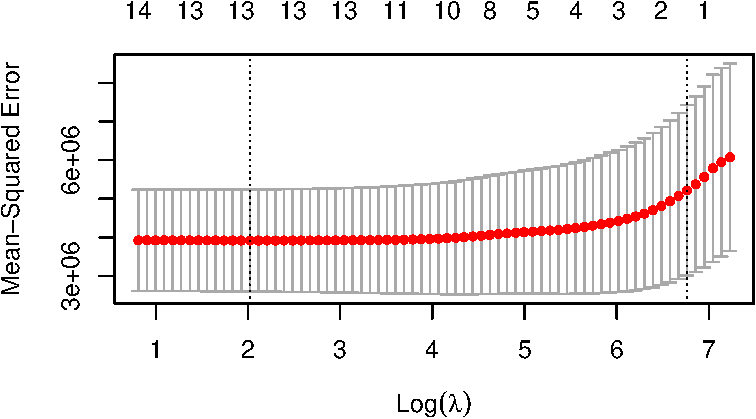
\includegraphics{Final_627_Tshiani_files/figure-pdf/unnamed-chunk-10-1.pdf}

\begin{itemize}
\tightlist
\item
  Show the result and identify whether \texttt{lambda-min} or
  \texttt{lambda.1se} has fewer non-zero variables?
\end{itemize}

\begin{Shaded}
\begin{Highlighting}[]
\FunctionTok{coef}\NormalTok{(lasso\_cv, }\AttributeTok{s =} \StringTok{"lambda.min"}\NormalTok{)}
\end{Highlighting}
\end{Shaded}

\begin{verbatim}
15 x 1 sparse Matrix of class "dgCMatrix"
                                 s0
(Intercept)           -2.512681e+03
ADM_RATE              -1.557644e+03
AVGFACSAL              5.584929e-01
CONTROLPublic         -8.723086e+02
FIRST_GEN              4.484255e+03
GRAD_DEBT_MDN         -7.331234e-02
PCIP27                 2.267653e+04
PCT_ASIAN             -9.547093e+01
REGIONGreat Lakes      1.052237e+02
REGIONMid-East        -4.603852e+02
REGIONNew England     -4.555186e+02
REGIONPLains           2.420369e+02
REGIONRocky Mountains  .           
REGIONSoutheast        2.121505e+02
REGIONSouthwest       -6.959190e+01
\end{verbatim}

\begin{Shaded}
\begin{Highlighting}[]
\FunctionTok{coef}\NormalTok{(lasso\_cv, }\AttributeTok{s =} \StringTok{"lambda.1se"}\NormalTok{)}
\end{Highlighting}
\end{Shaded}

\begin{verbatim}
15 x 1 sparse Matrix of class "dgCMatrix"
                                 s0
(Intercept)           -1187.7901159
ADM_RATE                  .        
AVGFACSAL                 0.1990341
CONTROLPublic             .        
FIRST_GEN                 .        
GRAD_DEBT_MDN             .        
PCIP27                    .        
PCT_ASIAN                 .        
REGIONGreat Lakes         .        
REGIONMid-East            .        
REGIONNew England         .        
REGIONPLains              .        
REGIONRocky Mountains     .        
REGIONSoutheast           .        
REGIONSouthwest           .        
\end{verbatim}

lambda-min has fewer zero variables.

\begin{itemize}
\tightlist
\item
  Show the coefficients for \texttt{lambda.1se} and discuss which were
  driven to zero if any.
\end{itemize}

\begin{Shaded}
\begin{Highlighting}[]
\FunctionTok{coef}\NormalTok{(lasso\_cv, }\AttributeTok{s =} \StringTok{"lambda.1se"}\NormalTok{)}
\end{Highlighting}
\end{Shaded}

\begin{verbatim}
15 x 1 sparse Matrix of class "dgCMatrix"
                                 s0
(Intercept)           -1187.7901159
ADM_RATE                  .        
AVGFACSAL                 0.1990341
CONTROLPublic             .        
FIRST_GEN                 .        
GRAD_DEBT_MDN             .        
PCIP27                    .        
PCT_ASIAN                 .        
REGIONGreat Lakes         .        
REGIONMid-East            .        
REGIONNew England         .        
REGIONPLains              .        
REGIONRocky Mountains     .        
REGIONSoutheast           .        
REGIONSouthwest           .        
\end{verbatim}

there pratically all were driven to zero except for AVGFACSAL.

\begin{itemize}
\tightlist
\item
  Do any of the +/- signs of the coefficients for the variables surprise
  you? using the labmda-min method, i would say a suprising result is
  colleges with a higher percentage of first-gen students have a higher
  endowement because i would expect the college to be spending the extra
  money on first-gen scholarships rather than the endowement.
\end{itemize}

What is the cross-validated predicted MSE from the model?

\begin{Shaded}
\begin{Highlighting}[]
\NormalTok{lasso\_cv}\SpecialCharTok{$}\NormalTok{cvm[lasso\_cv}\SpecialCharTok{$}\NormalTok{lambda }\SpecialCharTok{==}\NormalTok{ lasso\_cv}\SpecialCharTok{$}\NormalTok{lambda}\FloatTok{.1}\NormalTok{se]}
\end{Highlighting}
\end{Shaded}

\begin{verbatim}
[1] 5213701
\end{verbatim}

\subsection{Principal components.}\label{principal-components.}

Calculate the principal components using the \texttt{X} model matrix you
created earlier, with scaling, and show the scree plot.

\begin{Shaded}
\begin{Highlighting}[]
\NormalTok{pca }\OtherTok{\textless{}{-}} \FunctionTok{prcomp}\NormalTok{(x, }\AttributeTok{scale. =} \ConstantTok{TRUE}\NormalTok{)}
\FunctionTok{summary}\NormalTok{(pca)}
\end{Highlighting}
\end{Shaded}

\begin{verbatim}
Importance of components:
                          PC1    PC2     PC3     PC4     PC5     PC6     PC7
Standard deviation     1.6527 1.2569 1.17102 1.12916 1.08923 1.05543 1.01847
Proportion of Variance 0.1951 0.1128 0.09795 0.09107 0.08474 0.07957 0.07409
Cumulative Proportion  0.1951 0.3080 0.40590 0.49698 0.58172 0.66129 0.73538
                           PC8     PC9    PC10    PC11    PC12    PC13    PC14
Standard deviation     0.98138 0.90128 0.81662 0.74145 0.63683 0.51380 0.20775
Proportion of Variance 0.06879 0.05802 0.04763 0.03927 0.02897 0.01886 0.00308
Cumulative Proportion  0.80417 0.86219 0.90982 0.94909 0.97806 0.99692 1.00000
\end{verbatim}

\begin{Shaded}
\begin{Highlighting}[]
\FunctionTok{plot}\NormalTok{(pca, }\AttributeTok{type =} \StringTok{"l"}\NormalTok{)}
\end{Highlighting}
\end{Shaded}

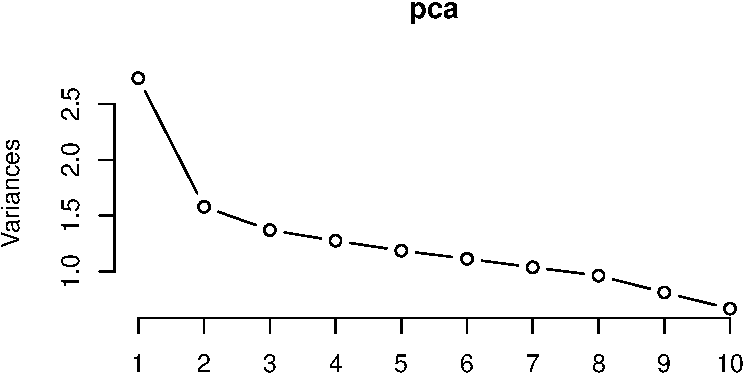
\includegraphics{Final_627_Tshiani_files/figure-pdf/unnamed-chunk-15-1.pdf}

\begin{itemize}
\tightlist
\item
  Interpret the scree plot
\end{itemize}

the line gradually flattens after 2 but not quite flat. i would still
recomment using 2-3 PCA components.

Given the scree plot, choose to create \textbf{either} a PCR \textbf{or}
a PLSR model.

I choose PSLR

\begin{Shaded}
\begin{Highlighting}[]
\FunctionTok{library}\NormalTok{(pls)}
\end{Highlighting}
\end{Shaded}

\begin{verbatim}

Attaching package: 'pls'
\end{verbatim}

\begin{verbatim}
The following object is masked from 'package:stats':

    loadings
\end{verbatim}

\begin{Shaded}
\begin{Highlighting}[]
\FunctionTok{set.seed}\NormalTok{(}\DecValTok{123}\NormalTok{)}
\NormalTok{plsr\_model }\OtherTok{\textless{}{-}} \FunctionTok{plsr}\NormalTok{(ENDOWBEGIN }\SpecialCharTok{\textasciitilde{}}\NormalTok{ ., }\AttributeTok{data =}\NormalTok{ college2, }\AttributeTok{scale =} \ConstantTok{TRUE}\NormalTok{, }\AttributeTok{validation =} \StringTok{"CV"}\NormalTok{)}
\FunctionTok{validationplot}\NormalTok{(plsr\_model, }\AttributeTok{val.type =} \StringTok{"MSEP"}\NormalTok{)}
\end{Highlighting}
\end{Shaded}

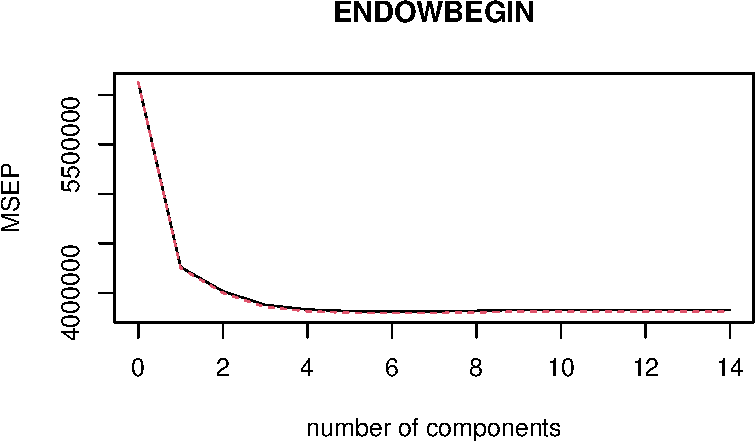
\includegraphics{Final_627_Tshiani_files/figure-pdf/unnamed-chunk-16-1.pdf}

\begin{Shaded}
\begin{Highlighting}[]
\FunctionTok{summary}\NormalTok{(plsr\_model)}
\end{Highlighting}
\end{Shaded}

\begin{verbatim}
Data:   X dimension: 918 14 
    Y dimension: 918 1
Fit method: kernelpls
Number of components considered: 14

VALIDATION: RMSEP
Cross-validated using 10 random segments.
       (Intercept)  1 comps  2 comps  3 comps  4 comps  5 comps  6 comps
CV            2475     2064     2004     1969     1957     1953     1952
adjCV         2475     2062     2000     1964     1953     1949     1948
       7 comps  8 comps  9 comps  10 comps  11 comps  12 comps  13 comps
CV        1953     1954     1957      1956      1956      1956      1956
adjCV     1949     1950     1952      1952      1952      1952      1952
       14 comps
CV         1956
adjCV      1952

TRAINING: % variance explained
            1 comps  2 comps  3 comps  4 comps  5 comps  6 comps  7 comps
X             19.01    27.26    32.67    40.05    46.87    54.21    58.84
ENDOWBEGIN    33.44    38.76    41.93    42.47    42.53    42.54    42.54
            8 comps  9 comps  10 comps  11 comps  12 comps  13 comps  14 comps
X             65.66    67.32     74.32     81.10     87.63     93.12    100.00
ENDOWBEGIN    42.54    42.54     42.54     42.54     42.54     42.54     42.54
\end{verbatim}

it takes 13 components to explain 90\% of variation in the x variables.
it takes 3 components to explain 40\% of components in the y variables.

Create the model with scaling and K=10 fold cross-validation. (Use seed
123).

How many principal components are

\begin{itemize}
\tightlist
\item
  Needed to explain 90\% of the total variation \emph{among
  X-variables}?
\item
  Needed to explain 40\% of the total variation \emph{of the response},
  \texttt{ENDOWBEGIN}?
\item
  What is the optimal number of PCs based on adjusted Cross-Validation
  RMSEP?
\item
  What is the adjusted Cross Validation MSEP for the optimal number of
  PCs
\item
  Show the validation plot.
\end{itemize}

\begin{Shaded}
\begin{Highlighting}[]
\FunctionTok{validationplot}\NormalTok{(plsr\_model, }\AttributeTok{val.type =} \StringTok{"RMSEP"}\NormalTok{)}
\end{Highlighting}
\end{Shaded}

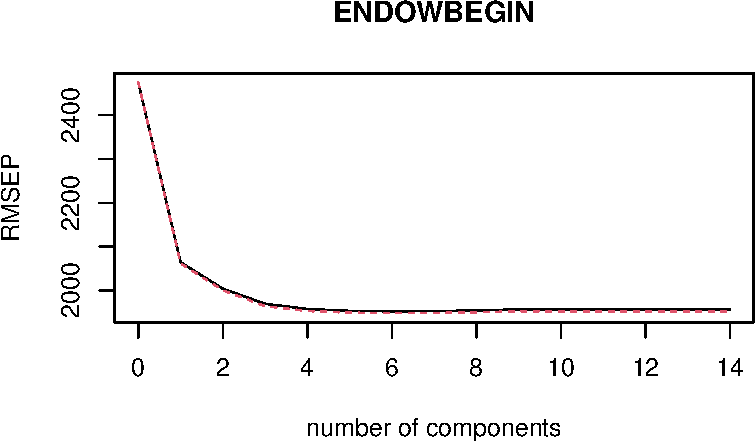
\includegraphics{Final_627_Tshiani_files/figure-pdf/unnamed-chunk-18-1.pdf}

optimal number of CVs are around 3-4

\subsection{Summary}\label{summary}

Create a summary table showing the method, the MSE, and the number of
predictors.

\begin{itemize}
\tightlist
\item
  Recommend a model for predicting \texttt{ENDOWBEGIN} for new
  observations and explain your choice.
\end{itemize}

\begin{longtable}[]{@{}lcc@{}}
\toprule\noalign{}
Method & Predicted MSE & Number of Predictors \\
\midrule\noalign{}
\endhead
\bottomrule\noalign{}
\endlastfoot
Linear Model (Reduced) & & \\
LASSO lambda.1se & & \\
PCR & & \\
PLSR & & \\
\end{longtable}

\begin{Shaded}
\begin{Highlighting}[]
\FunctionTok{library}\NormalTok{(tibble)}
\FunctionTok{library}\NormalTok{(boot)}
\FunctionTok{library}\NormalTok{(glmnet)}
\FunctionTok{library}\NormalTok{(pls)}

\CommentTok{\# 1. Reduced Linear Model (lm\_full assumed to be fitted on college2)}
\FunctionTok{set.seed}\NormalTok{(}\DecValTok{123}\NormalTok{)}
\NormalTok{cv\_lm }\OtherTok{\textless{}{-}} \FunctionTok{cv.glm}\NormalTok{(college2, lm\_full, }\AttributeTok{K =} \DecValTok{10}\NormalTok{)}
\NormalTok{mse\_lm }\OtherTok{\textless{}{-}}\NormalTok{ cv\_lm}\SpecialCharTok{$}\NormalTok{delta[}\DecValTok{1}\NormalTok{]}
\NormalTok{num\_lm }\OtherTok{\textless{}{-}} \FunctionTok{length}\NormalTok{(}\FunctionTok{coef}\NormalTok{(lm\_full)) }\SpecialCharTok{{-}} \DecValTok{1}  \CommentTok{\# exclude intercept}

\CommentTok{\# 2. LASSO (lambda.1se from lasso\_cv)}
\NormalTok{mse\_lasso }\OtherTok{\textless{}{-}}\NormalTok{ lasso\_cv}\SpecialCharTok{$}\NormalTok{cvm[lasso\_cv}\SpecialCharTok{$}\NormalTok{lambda }\SpecialCharTok{==}\NormalTok{ lasso\_cv}\SpecialCharTok{$}\NormalTok{lambda}\FloatTok{.1}\NormalTok{se]}
\NormalTok{coef\_lasso }\OtherTok{\textless{}{-}} \FunctionTok{coef}\NormalTok{(lasso\_cv, }\AttributeTok{s =} \StringTok{"lambda.1se"}\NormalTok{)}
\NormalTok{num\_lasso }\OtherTok{\textless{}{-}} \FunctionTok{sum}\NormalTok{(coef\_lasso }\SpecialCharTok{!=} \DecValTok{0}\NormalTok{) }\SpecialCharTok{{-}} \DecValTok{1}  \CommentTok{\# exclude intercept}

\CommentTok{\# 3. PLSR (from plsr\_model)}
\NormalTok{rmsep\_plsr }\OtherTok{\textless{}{-}} \FunctionTok{RMSEP}\NormalTok{(plsr\_model, }\AttributeTok{estimate =} \StringTok{"adjCV"}\NormalTok{)}
\NormalTok{mse\_plsr }\OtherTok{\textless{}{-}} \FunctionTok{min}\NormalTok{(rmsep\_plsr}\SpecialCharTok{$}\NormalTok{val[}\DecValTok{1}\NormalTok{,}\DecValTok{1}\NormalTok{,}\SpecialCharTok{{-}}\DecValTok{1}\NormalTok{])  }\CommentTok{\# remove Comp 0}
\NormalTok{num\_plsr }\OtherTok{\textless{}{-}} \FunctionTok{which.min}\NormalTok{(rmsep\_plsr}\SpecialCharTok{$}\NormalTok{val[}\DecValTok{1}\NormalTok{,}\DecValTok{1}\NormalTok{,}\SpecialCharTok{{-}}\DecValTok{1}\NormalTok{])}

\CommentTok{\# Combine into a summary tibble}
\NormalTok{model\_summary }\OtherTok{\textless{}{-}} \FunctionTok{tibble}\NormalTok{(}
  \AttributeTok{Method =} \FunctionTok{c}\NormalTok{(}\StringTok{"Linear Model (Reduced)"}\NormalTok{, }
             \StringTok{"LASSO (lambda.1se)"}\NormalTok{, }
             \StringTok{"PLSR"}\NormalTok{),}
  \AttributeTok{Predicted\_MSE =} \FunctionTok{c}\NormalTok{(mse\_lm, mse\_lasso, mse\_plsr),}
  \AttributeTok{Num\_Predictors =} \FunctionTok{c}\NormalTok{(num\_lm, num\_lasso, num\_plsr)}
\NormalTok{)}

\CommentTok{\# Print table}
\NormalTok{model\_summary}
\end{Highlighting}
\end{Shaded}

\begin{verbatim}
# A tibble: 3 x 3
  Method                 Predicted_MSE Num_Predictors
  <chr>                          <dbl>          <dbl>
1 Linear Model (Reduced)      3875289.             14
2 LASSO (lambda.1se)          5213701.              1
3 PLSR                           1948.              6
\end{verbatim}

\subsection{Classification with SVM (Optional Extra Credit 4
points)}\label{classification-with-svm-optional-extra-credit-4-points}

We now want to predict whether a new college is Private or Public based
on the data in \texttt{college2}.

Tune a Support Vector Machine model to find the best cost and kernel.

\begin{itemize}
\tightlist
\item
  Use the range of costs in \texttt{seq(4.0,\ 6.0,\ 0.25)} and the
  linear and radial kernels.
\end{itemize}

What is the best cost value and the best kernel and the cross-validated
error rate?

Create a model with the best parameters

\begin{itemize}
\tightlist
\item
  How many support vectors are there?
\end{itemize}

Plot the results looking at \texttt{ADM\_RATE} and \texttt{AVGFACSAL}.

\begin{itemize}
\tightlist
\item
  Comment on the plot
\end{itemize}

\begin{Shaded}
\begin{Highlighting}[]
\FunctionTok{library}\NormalTok{(e1071)}
\FunctionTok{rm}\NormalTok{(svm)}
\end{Highlighting}
\end{Shaded}

\begin{verbatim}
Warning in rm(svm): object 'svm' not found
\end{verbatim}

\begin{Shaded}
\begin{Highlighting}[]
\CommentTok{\# Tune separately for linear and radial kernels}
\FunctionTok{set.seed}\NormalTok{(}\DecValTok{123}\NormalTok{)}
\NormalTok{svm\_linear }\OtherTok{\textless{}{-}} \FunctionTok{tune}\NormalTok{(}
\NormalTok{  svm, CONTROL }\SpecialCharTok{\textasciitilde{}}\NormalTok{ ADM\_RATE }\SpecialCharTok{+}\NormalTok{ AVGFACSAL,}
  \AttributeTok{data =}\NormalTok{ college2,}
  \AttributeTok{kernel =} \StringTok{"linear"}\NormalTok{,}
  \AttributeTok{ranges =} \FunctionTok{list}\NormalTok{(}\AttributeTok{cost =} \FunctionTok{seq}\NormalTok{(}\FloatTok{4.0}\NormalTok{, }\FloatTok{6.0}\NormalTok{, }\FloatTok{0.25}\NormalTok{))}
\NormalTok{)}

\FunctionTok{set.seed}\NormalTok{(}\DecValTok{123}\NormalTok{)}
\NormalTok{svm\_radial }\OtherTok{\textless{}{-}} \FunctionTok{tune}\NormalTok{(}
\NormalTok{  svm, CONTROL }\SpecialCharTok{\textasciitilde{}}\NormalTok{ ADM\_RATE }\SpecialCharTok{+}\NormalTok{ AVGFACSAL,}
  \AttributeTok{data =}\NormalTok{ college2,}
  \AttributeTok{kernel =} \StringTok{"radial"}\NormalTok{,}
  \AttributeTok{ranges =} \FunctionTok{list}\NormalTok{(}\AttributeTok{cost =} \FunctionTok{seq}\NormalTok{(}\FloatTok{4.0}\NormalTok{, }\FloatTok{6.0}\NormalTok{, }\FloatTok{0.25}\NormalTok{))}
\NormalTok{)}

\CommentTok{\# Extract best cost and error for linear}
\NormalTok{best\_cost\_linear }\OtherTok{\textless{}{-}}\NormalTok{ svm\_linear}\SpecialCharTok{$}\NormalTok{best.parameters}\SpecialCharTok{$}\NormalTok{cost}
\NormalTok{best\_error\_linear }\OtherTok{\textless{}{-}}\NormalTok{ svm\_linear}\SpecialCharTok{$}\NormalTok{best.performance}

\CommentTok{\# Extract best cost and error for radial}
\NormalTok{best\_cost\_radial }\OtherTok{\textless{}{-}}\NormalTok{ svm\_radial}\SpecialCharTok{$}\NormalTok{best.parameters}\SpecialCharTok{$}\NormalTok{cost}
\NormalTok{best\_error\_radial }\OtherTok{\textless{}{-}}\NormalTok{ svm\_radial}\SpecialCharTok{$}\NormalTok{best.performance}

\CommentTok{\# Determine overall best kernel and cost}
\ControlFlowTok{if}\NormalTok{ (best\_error\_linear }\SpecialCharTok{\textless{}}\NormalTok{ best\_error\_radial) \{}
\NormalTok{  best\_kernel }\OtherTok{\textless{}{-}} \StringTok{"linear"}
\NormalTok{  best\_cost }\OtherTok{\textless{}{-}}\NormalTok{ best\_cost\_linear}
\NormalTok{  best\_error }\OtherTok{\textless{}{-}}\NormalTok{ best\_error\_linear}
\NormalTok{\} }\ControlFlowTok{else}\NormalTok{ \{}
\NormalTok{  best\_kernel }\OtherTok{\textless{}{-}} \StringTok{"radial"}
\NormalTok{  best\_cost }\OtherTok{\textless{}{-}}\NormalTok{ best\_cost\_radial}
\NormalTok{  best\_error }\OtherTok{\textless{}{-}}\NormalTok{ best\_error\_radial}
\NormalTok{\}}

\CommentTok{\# Print results}
\FunctionTok{cat}\NormalTok{(}\StringTok{"Best kernel:"}\NormalTok{, best\_kernel, }\StringTok{"}\SpecialCharTok{\textbackslash{}n}\StringTok{"}\NormalTok{)}
\end{Highlighting}
\end{Shaded}

\begin{verbatim}
Best kernel: radial 
\end{verbatim}

\begin{Shaded}
\begin{Highlighting}[]
\FunctionTok{cat}\NormalTok{(}\StringTok{"Best cost:"}\NormalTok{, best\_cost, }\StringTok{"}\SpecialCharTok{\textbackslash{}n}\StringTok{"}\NormalTok{)}
\end{Highlighting}
\end{Shaded}

\begin{verbatim}
Best cost: 4 
\end{verbatim}

\begin{Shaded}
\begin{Highlighting}[]
\FunctionTok{cat}\NormalTok{(}\StringTok{"Cross{-}validated error rate:"}\NormalTok{, best\_error, }\StringTok{"}\SpecialCharTok{\textbackslash{}n}\StringTok{"}\NormalTok{)}
\end{Highlighting}
\end{Shaded}

\begin{verbatim}
Cross-validated error rate: 0.3225036 
\end{verbatim}

\begin{Shaded}
\begin{Highlighting}[]
\FunctionTok{library}\NormalTok{(e1071)}
\NormalTok{final\_svm }\OtherTok{\textless{}{-}} \FunctionTok{svm}\NormalTok{(CONTROL }\SpecialCharTok{\textasciitilde{}}\NormalTok{ ADM\_RATE }\SpecialCharTok{+}\NormalTok{ AVGFACSAL, }\AttributeTok{data =}\NormalTok{ college2,}
                 \AttributeTok{kernel =} \StringTok{"radial"}\NormalTok{, }\AttributeTok{cost =} \DecValTok{4}\NormalTok{)}
\end{Highlighting}
\end{Shaded}

\begin{Shaded}
\begin{Highlighting}[]
\NormalTok{final\_svm}
\end{Highlighting}
\end{Shaded}

\begin{verbatim}

Call:
svm(formula = CONTROL ~ ADM_RATE + AVGFACSAL, data = college2, kernel = "radial", 
    cost = 4)


Parameters:
   SVM-Type:  C-classification 
 SVM-Kernel:  radial 
       cost:  4 

Number of Support Vectors:  617
\end{verbatim}

617 support vectors

\begin{Shaded}
\begin{Highlighting}[]
\FunctionTok{plot}\NormalTok{(final\_svm, }\AttributeTok{data =}\NormalTok{ college2[, }\FunctionTok{c}\NormalTok{(}\StringTok{"ADM\_RATE"}\NormalTok{, }\StringTok{"AVGFACSAL"}\NormalTok{, }\StringTok{"CONTROL"}\NormalTok{)],}
     \AttributeTok{main =} \StringTok{"SVM: ADM\_RATE vs AVGFACSAL"}\NormalTok{)}
\end{Highlighting}
\end{Shaded}

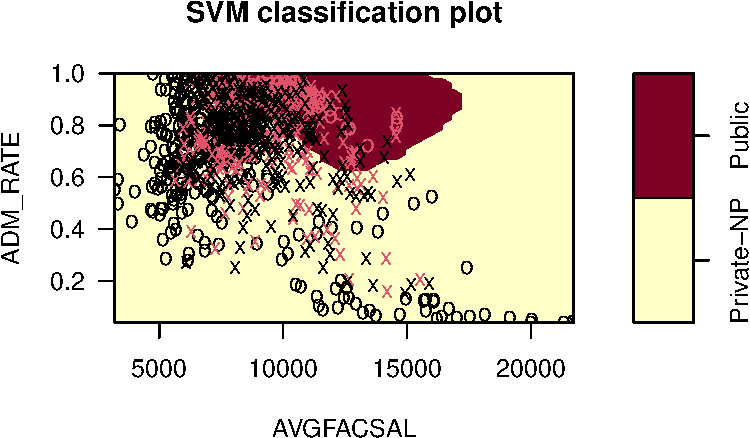
\includegraphics{Final_627_Tshiani_files/figure-pdf/unnamed-chunk-23-1.pdf}



\end{document}
